\documentclass[11pt]{article}
\usepackage[margin=1in]{geometry}
\usepackage{amsmath,amssymb,amsthm}
\usepackage{booktabs}
\usepackage{tikz}
\usetikzlibrary{arrows.meta,decorations.markings}
\usepackage[colorlinks=true,linkcolor=blue!50!black,citecolor=green!40!black,urlcolor=blue!60!black]{hyperref}

% ---------------------------------------------------------------- notation (as in topvertex_notes.tex)
\newcommand{\Z}{\mathbb{Z}}
\newcommand{\Q}{\mathbb{Q}}
\newcommand{\R}{\mathbb{R}}
\newcommand{\C}{\mathbb{C}}
\newcommand{\PP}{\mathbb{P}}
\newcommand{\CO}{\mathcal{O}}
\newcommand{\hatw}{\widehat{\omega}}
\newcommand{\topvertex}{\texttt{topvertex}}

\title{\vspace{-2.5em}Curve counting on toric Calabi-Yau threefolds:\\ a short summary of the invariants}
\author{A note accompanying the Python package \texttt{topvertex}}
\date{\vspace{-2.5em}}

\begin{document}
\maketitle

%=====================================================================================
\section{Introduction and summary}\label{sec:intro}
%=====================================================================================

The package \topvertex{} takes a lattice polygon $P\subset\R^2$ with a unimodular triangulation
$T$ and returns a power series $Z_T(q,Q)=1+\ldots$, together with a table of integers $n^g_\beta$
(see the main notes \cite{notes} for the algorithm). In this note we summarize, informally and
without proofs, what these quantities mean. The triangulated polygon encodes a complex
3-dimensional manifold $X_T$, a \textit{toric Calabi-Yau threefold}, and $Z_T$ is a generating
function of numbers that ``count'' holomorphic curves in $X_T$. The different ways to make
sense of such a count lead to the Gromov-Witten (GW), Gopakumar-Vafa (GV), Donaldson-Thomas (DT)
and Pandharipande-Thomas (PT) invariants, listed in Table \ref{tab:summary} (see \cite{PT13}
for a review). For a toric Calabi-Yau threefold all
four sets of numbers turn out to carry the same information, and $Z_T$ is their common
generating function. A change of the triangulation of a fixed polygon changes the invariants in
a simple and explicit way, given by the formula (\ref{flop-gv}) below. The geometry of $X_T$ is
reviewed in Section \ref{sec:geometry}, the invariants and their relations are described in
Sections \ref{sec:invariants} and \ref{sec:relations}, and a change of the triangulation is
considered in Section \ref{sec:flops}.

\begin{table}[ht]
\centering\small
\begin{tabular}{lllll}
\toprule
invariant & labelled by & values & what is ``counted'' & invariant of \\
\midrule
GW, $N_{g,\beta}$ & $g\geq 0$, $\beta$ & $\Q$ & holomorphic maps $\Sigma_g\rightarrow X$ &
symplectic manifold $(X,\omega)$\\
GV, $n^g_\beta$ & $g\geq 0$, $\beta$ & $\Z$ & BPS states of wrapped M2-branes &
\quad up to deformations\\[2pt]
DT, $I_{n,\beta}$ & $n\in\Z$, $\beta$ & $\Z$ & curves and points cut out by equations &
complex manifold $X$\\
PT, $P_{n,\beta}$ & $n\in\Z$, $\beta$ & $\Z$ & curves with points on them &
\quad up to deformations\\
\bottomrule
\end{tabular}
\caption{The curve counting invariants of a Calabi-Yau threefold $X$, with
$0\neq\beta\in H_2(X,\Z)$.}\label{tab:summary}
\end{table}

%=====================================================================================
\section{The threefold behind the picture}\label{sec:geometry}
%=====================================================================================

In this section we review how a triangulated polygon determines a threefold, and which of its
features depend on the polygon only. Each lattice point $\omega=(x,y)$ of $P$ is lifted to
$\hatw=(x,y,1)\in\Z^3$. The cones over the triangles of $T$ form a fan, and $X_T$ is the
corresponding toric variety, with an action of the torus $(\C^*)^3$. Unimodularity of the
triangles means that $X_T$ is smooth. The fact that all $\hatw$ lie in one plane means that $X_T$
has a nowhere vanishing holomorphic 3-form, which is the \textit{Calabi-Yau} condition, and
forces $X_T$ to be non-compact. The triangulation is regular precisely when $X_T$ is quasi-projective, in which case the heights determine a K\"ahler class.
The triangles correspond to the fixed points of the torus action, and the interior segments
$\tau$ to compact holomorphic curves $C_\tau\cong\PP^1$. Polygons related by an affine
transformation preserving the lattice $\Z^2$ give isomorphic threefolds.

The following data are the same for all unimodular triangulations of a given polygon $P$.
First, the group of curve classes: $H_2(X_T,\Z)\cong L:=\{l\in\Z^N:\sum_i l_i\hatw_i=0\}$, where
$N$ is the number of lattice points of $P$, and the class of $C_\tau$ is the relation vector
$l_\tau$ of \cite{notes}. Second, the Euler characteristic $\chi(X_T)$, which is equal to the
number of triangles, i.e.\ to twice the area of $P$. Finally, the singular affine toric variety
$X_P$ of the cone over $P$, for example the conifold $\{xy=zw\}\subset\C^4$ when $P$ is the unit
square. Each $X_T$ is a \textit{crepant resolution} of $X_P$, that is a resolution of the
singularities with a trivial canonical bundle. What does depend on $T$ is the set of \textit{effective}
classes, i.e.\ the classes of holomorphic curves, which are the non-negative integral
combinations of the $l_\tau$.

%=====================================================================================
\section{The invariants}\label{sec:invariants}
%=====================================================================================

In this section we describe the invariants one by one. Let $X$ be a Calabi-Yau threefold.

\paragraph{Gromov-Witten invariants.} Informally, $N_{g,\beta}$ is the number of holomorphic maps
$f:\Sigma_g\rightarrow X$ from Riemann surfaces of genus $g$, such that the image has class $\beta$, counted up to reparametrizations of
$\Sigma_g$. For a Calabi-Yau threefold such maps are expected to be isolated for all $g$ and
$\beta$, which is why one obtains numbers without imposing any conditions on the curves. A map
with a finite group of automorphisms is counted with the weight $1/|\mathrm{Aut}|$, and
therefore the numbers are rational. The GW
invariants are invariants of the symplectic manifold $(X,\omega)$. They do not change under
continuous deformations of the symplectic form $\omega$ and of the compatible (almost) complex
structure. In particular, for a K\"ahler manifold they depend neither on the complex structure
nor on the K\"ahler class, as long as these are varied without making $X$ singular.

\paragraph{The topological string.} Physically, the GW invariants are computed by the A-model
topological string theory on $X$, a theory of maps from 2-dimensional surfaces to $X$ in which
the path integral reduces to a sum over holomorphic maps (see \cite{Marino} for a review). Its
partition function is
\begin{equation}\label{top-string-Z}
Z=\exp\Big(\sum_{g\geq0}g_s^{2g-2}F_g(Q)\Big),\qquad F_g(Q)=\sum_{\beta\neq0}N_{g,\beta}\,Q^\beta,
\end{equation}
where $g_s$ is the string coupling and $Q^\beta=e^{-t_\beta}$, with $t_\beta$ being the
(complexified) area of a curve of class $\beta$. The theory is sensitive to the K\"ahler class
of $X$ only through the variables $Q$, and is not sensitive to the complex structure. The series
computed by \topvertex{} is (\ref{top-string-Z}) for $X=X_T$ with $q=e^{ig_s}$. The topological
vertex was derived in \cite{AKMV} from a duality with Chern-Simons theory, and was proved to
agree with the mathematical definition of the GW invariants in \cite{LLLZ,MOOP}. Since $X_T$ is
non-compact, its invariants are in general \textit{defined} by localization, i.e.\ as sums of
contributions of the curves fixed by the torus action.

\paragraph{Gopakumar-Vafa invariants.} In M-theory on $X\times\R^5$ an M2-brane wrapping a
holomorphic curve of class $\beta$ is a charged particle in five dimensions. The number
$n^g_\beta$ is a signed count of the supersymmetric (BPS) states of such particles, where $g$
labels their spin content. It was argued in \cite{GV} that
\begin{equation}\label{gv-formula}
\log Z=\sum_{\beta\neq0}\sum_{g\geq0}\sum_{k\geq1}n^g_\beta\,\frac{(-1)^{g-1}}{k}\,[k]^{2g-2}\,Q^{k\beta},
\qquad [k]:=q^{k/2}-q^{-k/2}.
\end{equation}
Mathematically, (\ref{gv-formula}) can be taken as the definition of $n^g_\beta$ in terms of
$N_{g,\beta}$, and this is how \topvertex{} computes them. The non-trivial statements are then
that $n^g_\beta$ are integers and that $n^g_\beta=0$ for large $g$ at fixed $\beta$. This was
proved for toric Calabi-Yau threefolds in \cite{Peng,Kon}, and the integrality for general
symplectic Calabi-Yau manifolds of real dimension 6 in \cite{IP}. Informally, $n^0_\beta$ is the
number of rational curves of class $\beta$ with the contributions of multiple covers removed.
Being a reorganization of the GW invariants, the GV invariants are invariant under the same
deformations.

\paragraph{Donaldson-Thomas and Pandharipande-Thomas invariants.} Here a curve is described not
by a map but by equations. The integer $I_{n,\beta}$ is a virtual number of 1-dimensional
subschemes $S\subset X$ of class $\beta$ with the holomorphic Euler characteristic
$\chi(\CO_S)=n$ \cite{MNOP}. Such $S$ is a curve, possibly with multiplicities, together
with a finite number of points, which can lie on the curve or away from it. The PT invariants
$P_{n,\beta}$ similarly count \textit{stable pairs} \cite{PT}, which informally are curves with a
finite number of points lying on them. We denote the generating functions by
$Z_\text{DT}(p,Q)=\sum_{n,\beta}I_{n,\beta}\,p^nQ^\beta$ and
$Z_\text{PT}(p,Q)=\sum_{n,\beta}P_{n,\beta}\,p^nQ^\beta$, where the sums include $\beta=0$. Both
are invariants of the complex manifold $X$, unchanged under deformations of its complex
structure, and no choice of a K\"ahler class enters the definition. For $X=X_T$ the subschemes
fixed by the torus action are described by 3-dimensional partitions (piles of boxes) placed at
the triangles \cite{ORV,MNOP}, and the vertex $C_{\lambda_1\lambda_2\lambda_3}(q)$ is, up to
normalization, the generating function of the 3-dimensional partitions with the asymptotic
shapes $\lambda_1,\lambda_2,\lambda_3$.

%=====================================================================================
\section{Relations}\label{sec:relations}
%=====================================================================================

In this section we list the relations between the invariants. Taken together, for $X=X_T$ they
state that
\begin{equation}\label{all-equal}
Z_T(q,Q)=\exp\Big(\sum_{g\geq0}g_s^{2g-2}F_g(Q)\Big)=Z_\text{PT}(p,Q)=
\frac{Z_\text{DT}(p,Q)}{M(q)^{\chi(X_T)}},\qquad q=e^{ig_s}=-p,
\end{equation}
where $M(q):=\prod_{k\geq1}(1-q^k)^{-k}$. The last equality is the DT/PT correspondence,
conjectured in \cite{MNOP,PT} and proved for projective Calabi-Yau threefolds in
\cite{Bridgeland-hall}. The denominator is the part of $Z_\text{DT}$ with $\beta=0$, which counts
points. The middle equality is the GW/DT correspondence conjectured in \cite{MNOP} and proved
for toric threefolds in \cite{MOOP}. The GW and GV invariants can be recovered from each other
directly from (\ref{gv-formula}), for example $N_{0,\beta}=\sum_{k|\beta}n^0_{\beta/k}/k^3$.
Finally, exponentiating (\ref{gv-formula}) one obtains the product formula
\begin{equation}\label{gv-product}
Z_T(q,Q)=\prod_{\beta\neq0}\Big[\prod_{k\geq1}\big(1-q^kQ^\beta\big)^{k\,n^0_\beta}\;
\prod_{g\geq1}\prod_{j=0}^{2g-2}\big(1-q^{g-1-j}Q^\beta\big)^{(-1)^{g+j}\binom{2g-2}{j}n^g_\beta}\Big],
\end{equation}
which relates the GV invariants to the PT invariants. For the resolved conifold, with the only
non-zero invariant $n^0_{[C]}=1$, it reads
\begin{equation}\label{conifold-Z}
Z_T(q,Q)=\prod_{k\geq1}\big(1-q^kQ\big)^k .
\end{equation}

Note that, unlike (\ref{gv-formula}), the GW/DT correspondence is not a relation between
individual numbers. For a fixed $\beta$, the coefficient of $Q^\beta$ in $Z_\text{PT}$ is the series
$\sum_nP_{n,\beta}\,p^n$ with finitely many negative powers of $p$. It is the expansion at $p=0$ of
a rational function of $p$, invariant under $p\rightarrow1/p$. The GW invariants are obtained by
substituting $p=-e^{ig_s}$ into this rational function and expanding it in $g_s$, that is by
expanding it at a different point, $p=-1$. Therefore each $N_{g,\beta}$ depends on infinitely
many of the integers $P_{n,\beta}$. For example, the coefficient of $Q$ in (\ref{conifold-Z}) is
\begin{equation}\label{conifold-gw-pt}
\sum_{n\geq1}(-1)^{n-1}n\,p^n=\frac{p}{(1+p)^2}=\frac{1}{\big(2\sin\frac{g_s}{2}\big)^2}=
\frac{1}{g_s^2}+\frac{1}{12}+\frac{g_s^2}{240}+\ldots,
\end{equation}
so that $P_{n,[C]}=(-1)^{n-1}n$ for $n\geq1$, while $N_{0,[C]}=1$, $N_{1,[C]}=1/12$,
$N_{2,[C]}=1/240$.

%=====================================================================================
\section{Change of the triangulation}\label{sec:flops}
%=====================================================================================

In this section we describe how the invariants depend on the triangulation $T$ of a fixed
polygon $P$. Any two unimodular triangulations of $P$ are related by a sequence of
\textit{flips} \cite{DLRS}. A flip replaces a diagonal $\tau$ of a parallelogram formed by two
adjacent triangles with the other diagonal $\tau'$ (Figure \ref{fig:flip}). An interior segment
$\tau$ can be flipped precisely when its framing in the sense of \cite{notes} is zero, that is
when $C_\tau$ has the normal bundle $\CO(-1)\oplus\CO(-1)$. Geometrically, a flip is a
\textit{flop}. The curve $C_\tau$ is contracted to a point, which produces a conifold
singularity, and the singularity is then resolved in the other way, by a new curve
$C_{\tau'}$. Since $X_T$ and $X_{T'}$ are not related by a continuous deformation through smooth
manifolds, the invariance properties of Section \ref{sec:invariants} do not apply, and the
invariants do change. With both groups of curve classes identified with $L$ as in
Section \ref{sec:geometry}, we have $l_{\tau'}=-l_\tau$, so that the new curve formally has a
negative area in terms of the old variables.

\begin{figure}[ht]
\begin{minipage}{0.5\textwidth}\centering
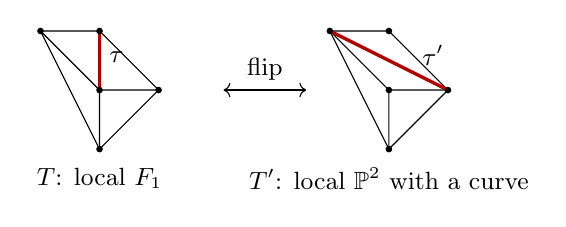
\begin{tikzpicture}[scale=0.75]
 \begin{scope}
 \draw (1,0)--(0,1)--(-1,1)--(0,-1)--cycle;
 \draw (0,0)--(1,0) (0,0)--(-1,1) (0,0)--(0,-1);
 \draw[very thick,red!70!black] (0,0)--(0,1);
 \foreach \p in {(0,0),(1,0),(0,1),(-1,1),(0,-1)} \fill \p circle (1.6pt);
 \node[right] at (0,0.55) {\small$\tau$};
 \node at (0,-1.5) {\small $T$: local $F_1$};
 \end{scope}
 \draw[<->] (2.1,0)--(3.5,0) node[midway,above] {\small flip};
 \begin{scope}[xshift=4.9cm]
 \draw (1,0)--(0,1)--(-1,1)--(0,-1)--cycle;
 \draw (0,0)--(1,0) (0,0)--(-1,1) (0,0)--(0,-1);
 \draw[very thick,red!70!black] (1,0)--(-1,1);
 \foreach \p in {(0,0),(1,0),(0,1),(-1,1),(0,-1)} \fill \p circle (1.6pt);
 \node[above right] at (0.4,0.25) {\small$\tau'$};
 \node at (0,-1.5) {\small $T'$: local $\PP^2$ with a curve};
 \end{scope}
\end{tikzpicture}
\end{minipage}\hfill
\begin{minipage}{0.46\textwidth}
\caption{The two unimodular triangulations of the polygon with corners
$(1,0),(0,1),(-1,1),(0,-1)$. On the left, $l_\tau=B$ is the class of the base of the Hirzebruch
surface $F_1$. On the right, the class of a line in $\PP^2$ is $H=B+F$, where $F$ is the class of
the fiber of $F_1$, and the class of the extra curve is $-B$.}\label{fig:flip}
\end{minipage}
\end{figure}

The change is, however, rather mild. Namely, for regular triangulations $T$ and $T'$
related by a flip of $\tau$ one has
\begin{equation}\label{flop-gv}
n^g_\beta(X_{T'})=n^g_\beta(X_T)\qquad\text{for all }g\text{ and all }\beta\in L\text{ not proportional to }l_\tau,
\end{equation}
while the only non-zero invariant on the line spanned by $l_\tau$ is $n^0_{l_\tau}(X_T)=1$,
which is replaced by $n^0_{-l_\tau}(X_{T'})=1$. Equivalently, in terms of the product formula
(\ref{gv-product}),
\begin{equation}\label{flop-Z}
\frac{Z_{T'}(q,Q)}{\prod_{k\geq1}(1-q^kQ^{-l_\tau})^k}=\frac{Z_T(q,Q)}{\prod_{k\geq1}(1-q^kQ^{l_\tau})^k}\,.
\end{equation}
Here both sides are power series in the monomials $Q^\beta$ with $\beta$ effective both in $X_T$
and in $X_{T'}$. In view of (\ref{all-equal}), the same statement holds for the GW, PT and DT
invariants. For the topological vertex the formula (\ref{flop-Z}) was proved in \cite{KM}. It is
a special case of general results, which do not require $X$ to be toric: for the GW invariants
in all genera \cite{LR}, and for the DT and PT invariants \cite{Toda-flop,Calabrese}.
Mathematically, all $X_T$ have equivalent derived categories of coherent sheaves, and the
invariants of $X_T$ and $X_{T'}$ count objects of this category that are stable in two different
senses \cite{Toda-flop,Calabrese}.

\paragraph{Example: local $\PP^1$.} The simplest example is the unit square with its two
triangulations $T$ and $T'$, given by the two diagonals. Both $X_T$ and $X_{T'}$ are the resolved
conifold, i.e.\ the total space of $\CO(-1)\oplus\CO(-1)\rightarrow\PP^1$, but the classes of the two
curves are opposite generators of $L\cong\Z$. With $Q:=Q^{l_\tau}$, the formula
(\ref{conifold-Z}) gives
\begin{equation}\label{conifold-flop}
Z_T(q,Q)=\prod_{k\geq1}\big(1-q^kQ\big)^k,\qquad Z_{T'}(q,Q)=\prod_{k\geq1}\big(1-q^kQ^{-1}\big)^k,
\end{equation}
and both sides of (\ref{flop-Z}) are equal to 1. The two series in (\ref{conifold-flop}) are
expansions at $Q=0$ and at $Q=\infty$, and it is instructive to compare them as functions of $Q$.
From (\ref{gv-formula}) and (\ref{conifold-gw-pt}), their free energies in the genus expansion
(\ref{top-string-Z}) are
\begin{equation}\label{conifold-Fg}
F_g(Q)=c_g\,\mathrm{Li}_{3-2g}(Q),\qquad F'_g(Q)=c_g\,\mathrm{Li}_{3-2g}(1/Q),\qquad
\mathrm{Li}_s(Q):=\sum_{k\geq1}\frac{Q^k}{k^s},
\end{equation}
where $c_0=1$, $c_1=1/12$, $c_2=1/240,\ldots$ are the coefficients in (\ref{conifold-gw-pt}). For
$g\geq2$ the function $\mathrm{Li}_{3-2g}(Q)$ is a rational function of $Q$ invariant under
$Q\rightarrow1/Q$, for example $\mathrm{Li}_{-1}(Q)=Q/(1-Q)^2$. Therefore $F_g$ and $F'_g$ are
expansions of the same function. For $g=0,1$ this is true only up to a polynomial in $\log(-Q)$:
\begin{equation}\label{polylog-inversion}
\mathrm{Li}_3(Q)-\mathrm{Li}_3(1/Q)=-\frac16\log^3(-Q)-\frac{\pi^2}{6}\log(-Q),\qquad
\mathrm{Li}_1(Q)-\mathrm{Li}_1(1/Q)=-\log(-Q).
\end{equation}
A cubic polynomial in the K\"ahler parameter $t=-\log Q$ in genus 0, and a linear one in genus 1,
have the form of the contributions of $\beta=0$ to the free energy, which are not included in
$Z_T$. For a compact Calabi-Yau threefold these contributions are given by the triple
intersection numbers and by the second Chern class, which change under a flop in a way that
compensates (\ref{polylog-inversion}) \cite{Witten-phases,AGM}. Physically, the K\"ahler cones of
the different $X_T$ are glued along their walls into a single space of K\"ahler parameters, and
the complete free energy is analytic across the walls. In this sense, in the general formula
(\ref{flop-Z}) the factors of the flopped curve also match, and $Z_T$ and $Z_{T'}$ are
expansions of the same function in two different regions.

\paragraph{Example: local $F_1$.} For the polygon in Figure \ref{fig:flip}, the relation
(\ref{flop-gv}) implies that the invariants of local $F_1$ in the classes $dB+dF$ coincide with
the invariants $3,-6,27,\ldots$ of local $\PP^2$ in degree $d$. We verified (\ref{flop-gv}) with
\topvertex{} for this polygon, for all classes up to a certain weight, including $g>0$.

%=====================================================================================
{\footnotesize
\begin{thebibliography}{99}\setlength{\itemsep}{-2pt}\setlength{\parsep}{0pt}
\bibitem{notes} \textit{The topological vertex as an algorithm: conventions and worked examples},
notes accompanying the Python package \texttt{topvertex}.
\bibitem{PT13} R.~Pandharipande, R.~P.~Thomas, \textit{13/2 ways of counting curves},
\texttt{arXiv:1111.1552}.
\bibitem{Marino} M.~Mari\~no, \textit{Chern-Simons theory and topological strings},
\texttt{arXiv:hep-th/0406005}.
\bibitem{AKMV} M.~Aganagic, A.~Klemm, M.~Mari\~no, C.~Vafa, \textit{The topological vertex},
\texttt{arXiv:hep-th/0305132}.
\bibitem{LLLZ} J.~Li, C.-C.~M.~Liu, K.~Liu, J.~Zhou, \textit{A mathematical theory of the
topological vertex},
\texttt{arXiv:math/0408426}.
\bibitem{MOOP} D.~Maulik, A.~Oblomkov, A.~Okounkov, R.~Pandharipande,
\textit{Gromov-Witten/Donaldson-Thomas correspondence for toric 3-folds},
\texttt{arXiv:0809.3976}.
\bibitem{GV} R.~Gopakumar, C.~Vafa, \textit{M-theory and topological strings I, II},
\texttt{arXiv:hep-th/9809187}, \texttt{arXiv:hep-th/9812127}.
\bibitem{Peng} P.~Peng, \textit{A simple proof of Gopakumar-Vafa conjecture for local toric
Calabi-Yau manifolds},
\texttt{arXiv:math/0410540}.
\bibitem{Kon} Y.~Konishi, \textit{Integrality of Gopakumar-Vafa invariants of toric Calabi-Yau
threefolds},
\texttt{arXiv:math/0504188}.
\bibitem{IP} E.-N.~Ionel, T.~H.~Parker, \textit{The Gopakumar-Vafa formula for symplectic
manifolds},
\texttt{arXiv:1306.1516}.
\bibitem{MNOP} D.~Maulik, N.~Nekrasov, A.~Okounkov, R.~Pandharipande, \textit{Gromov-Witten theory
and Donaldson-Thomas theory, I},
\texttt{arXiv:math/0312059}.
\bibitem{PT} R.~Pandharipande, R.~P.~Thomas, \textit{Curve counting via stable pairs in the
derived category},
\texttt{arXiv:0707.2348}.
\bibitem{ORV} A.~Okounkov, N.~Reshetikhin, C.~Vafa, \textit{Quantum Calabi-Yau and classical
crystals},
\texttt{arXiv:hep-th/0309208}.
\bibitem{Bridgeland-hall} T.~Bridgeland, \textit{Hall algebras and curve-counting invariants},
\texttt{arXiv:1002.4374}.
\bibitem{DLRS} J.~A.~De Loera, J.~Rambau, F.~Santos, \textit{Triangulations: structures for
algorithms and applications}, Springer, 2010.
\bibitem{KM} Y.~Konishi, S.~Minabe, \textit{Flop invariance of the topological vertex},
\texttt{arXiv:math/0601352}.
\bibitem{LR} A.-M.~Li, Y.~Ruan, \textit{Symplectic surgery and Gromov-Witten invariants of
Calabi-Yau 3-folds},
\texttt{arXiv:math/9803036}.
\bibitem{Toda-flop} Y.~Toda, \textit{Curve counting theories via stable objects II: DT/ncDT flop
formula},
\texttt{arXiv:0909.5129}.
\bibitem{Calabrese} J.~Calabrese, \textit{Donaldson-Thomas invariants and flops},
\texttt{arXiv:1111.1670}.
\bibitem{Witten-phases} E.~Witten, \textit{Phases of $N=2$ theories in two dimensions},
\texttt{arXiv:hep-th/9301042}.
\bibitem{AGM} P.~S.~Aspinwall, B.~R.~Greene, D.~R.~Morrison, \textit{Calabi-Yau moduli space,
mirror manifolds and spacetime topology change in string theory},
\texttt{arXiv:hep-th/9309097}.
\end{thebibliography}}

\end{document}
